
\section{Mạng Internet}
\label{sec:4.2}
Một trong những hệ thống liên mạng nổi trội nhất đó là mạng \textbf{Internet} (chú ý chữ I
viết hoa), đây là hệ thống mà bắt nguồn từ những dự án nghiên cứu từ những năm 1960 trở về
trước. Mục đích là phát triển khả năng kết nối nhiều mạng máy tính mà chúng có chức năng
như là một hệ thống kết nối không bị phá vỡ bởi những nguy cơ cục bộ. Hầu hết những công
việc ban đầu đều được tài trợ bởi chính phủ Mỹ thông qua Quỹ nghiên cứu Bộ quốc phòng Mỹ
(DARPA - được phát âm là ``DAR-pa''). Trải qua nhiều năm, sự phát triển của mạng Internet
thay đổi (thăng trầm) từ dự án quốc phòng tới dự án nghiên cứu mang tính chất học thuật,
và ngày nay nó được coi là một hệ thống thương mại mà có thể nối kết một tổ hợp các mạng
WAN, MAN, và LAN bao gồm hàng triệu máy tính.

\subsection*{Cấu trúc mạng Internet}
Về khía cạnh khái niệm, mạng Internet có thể được xem như là một tập hợp nhiều
\textbf{miền} (domains), mỗi miền bao gồm một mạng máy tính hay một liên mạng vừa và nhỏ được
điều hành bởi một tổ chức độc lập như một trường đại học, một công ty, hay cơ quan thuộc
chính phủ. Mỗi miền là một hệ thống tự trị (autonomous system) mà có thể được cấu hình với
yêu cầu về mức độ quyền hạn cục bộ. Nó có thể bao gồm một máy tính đơn hay một hệ thống
liên mạng phức tạp có thể bao gồm rất nhiều mạng LAN, MAN, hay thậm chí là mạng WAN.

Sự thành lập của các miền được giám sát bởi \textbf{ICANN (Internet Corporation for
  Assigned Names and Numbers)}, là một tổ chức phi lợi nhuận thực hiện việc thiết lập tên
cho các miền và gán các địa chỉ Internet, ta sẽ xem xét tới vấn đề này ngay sau
đây. Để thành lập một miền trên mạng Internet, miền đó trước tiên phải được đăng ký thông
qua các công ty, gọi là các nhà đăng ký mà đại diện cho tổ chức ICANN.


\begin{figure}[t]
  \begin{quotation}
    \noindent
    \textbf{Internet2} \vspace{0.3cm}
    \\
    Ngày nay mạng Internet đã thay đổi từ một dự án nghiên cứu thành một sản phẩm mang
    tính chất gia đình, cộng đồng nghiên cứu đã chuyển sang một dự án mang tên
    Internet2. Internet2 được mong đợi như là một hệ thống có tính chất học thuật và bao
    gồm rất nhiều các trường đại học làm việc công tác với ngày công nghiệp và chính
    phủ. Mục đích là kiểm soát việc nghiên cứu đối với các ứng dụng liên mạng yêu cầu độ
    rộng dải tần cao trong truyền thông, như hệ thống truy cập và điều khiển từ xa của
    những thiết bị đắt tiền như kính viễn vọng và những thiết bị chẩn đoán trong y tế. Một
    ví dụ của nghiên cứu này là việc thực hiện phẫu thuật từ xa thông qua bàn tay của rô
    bốt bắt chước các cử động của đôi bàn tay của một nhà phẫu thuật ngồi từ xa và quan
    sát bệnh nhân qua băng video. Bạn có thể xem thêm về Internet2 tại địa chỉ \url{
      http://www.internet2.org}
  \end{quotation}
\end{figure}


Khi một miền được đăng ký, nó có thể được gắn vào mạng Internet hiện tại thông qua một bộ
dẫn đường (router) mà kết nối một trong những mạng trong miền tới một mạng đã tồn tại trên
Internet. Bộ dẫn đường đặc biệt này thường được xem như là một cổng vào/ra (gateway) của
miền mà qua đó, nó đại diện cho cổng của miền ra phần còn lại của Internet. Xét trên góc
độ tầm nhìn, nó là một miền đơn lẻ, phần mạng của Internet nằm phía ngoài của cổng vào ra đôi
khi được gọi là đám mây (cloud).

\subsection*{Kết nối tới mạng Internet}

Để đơn giản hóa quá trình kết nối tới mạng Internet, rất nhiều công ty, được gọi là
\textbf{nhà cung cấp dịch vụ Internet (ISP)}, cho phép các khách hàng kết nối những miền
của họ ra ngoài Internet thông qua các thiết bị của ISP hay trở thành một phần của một
miền đã được thiết lập bởi ISP. Có lẽ những cách thức kết nối với chi phí ít tốn kém nhất
tới một ISP vẫn được sử dụng là thông qua các kết nối điện thoại được gọi là kết nối kiểu
quay số (dial-up). Bằng việc sử dụng theo cách thức này, một cá nhân có thể kết nối máy
tính của anh ta hay của cô ta tới đường thoại cục bộ và thực thi một gói phần mềm với
nhiệm vụ gọi đến một máy tính đặt tại ISP. Tại thời điểm đó, ISP cung cấp truy cập
Internet trong suốt thời gian gọi của điện thoại.


\begin{figure}[bth] 
  \centering \scalebox{0.45}{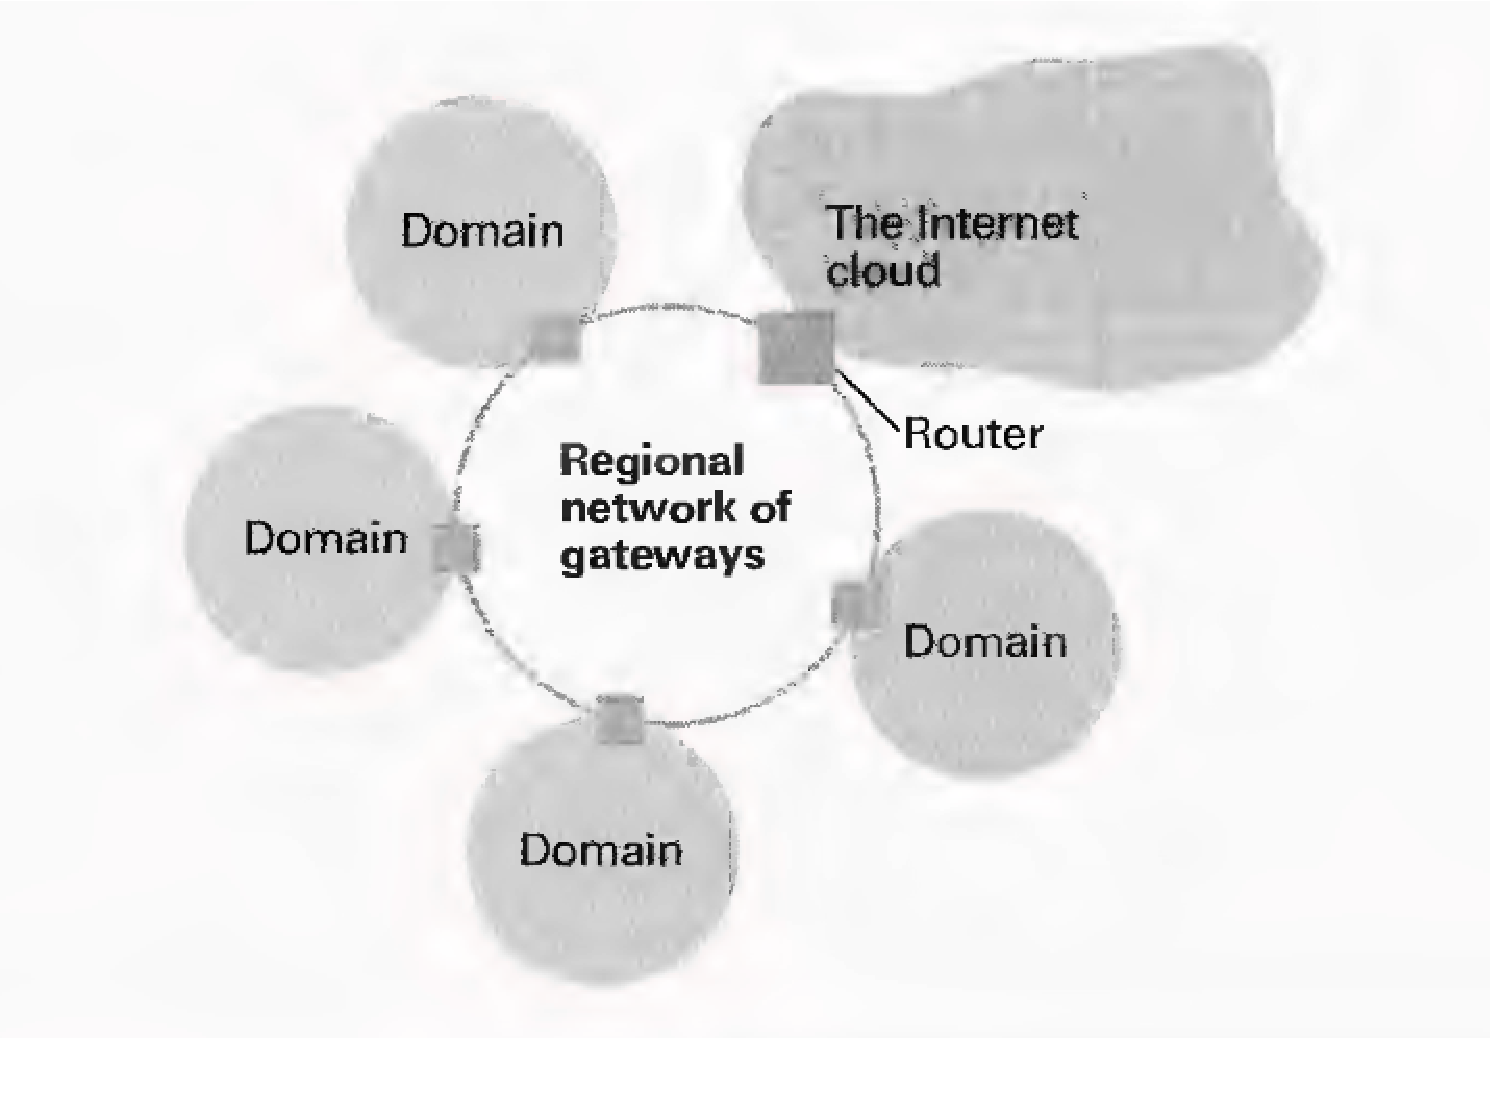
\includegraphics{ch5/fig47.pdf}}
  \caption{ Một cách thức kết nối điển hình tới mạng Internet}
  \label{fig:fig4.7}
\end{figure}

\subsection*{Đánh địa chỉ Internet}
Như đã giới thiệu trong Mục~\ref{sec:4.1}, một liên mạng cần phải được kết hợp với một hệ
thống địa chỉ liên mạng diện rộng mà sẽ gán một địa chỉ xác định cho mỗi máy tính trong hệ
thống. Trong Internet, những địa chỉ này được biết đến như là những \textbf{địa chỉ IP}
(Ký hiệu IP được viết tắt từ cụm “Internet Protocol”, khái niệm mà ta sẽ được giới thiệu
trong Mục~\ref{sec:4.4}). Mỗi địa chỉ IP là một bộ gồm 32 bít và trên thực tế cho đến ngày
nay địa chỉ IP đang trên đà tăng lên thành 128 bít (xem thảo luận về IPv6 trong phần
4.4). Mỗi địa chỉ 32 bít bao gồm hai phần: một phần xác định miền mà trong đó các máy tính
cư trú và một phần xác định mỗi máy tính cụ thể trong miền đó. Phần địa chỉ xác định miền,
được gọi là phần \textbf{định danh mạng}, được gán dưới sự kiểm soát của ICANN tại thời
điểm mà miền đó được đăng ký. Như vậy thông qua quá trình đăng ký này mà mỗi miền trong
mạng Internet được đảm bảo chắc chắn là có một định danh mạng là duy nhất. Phần địa chỉ
xác định một máy tính cụ thể trong miền được gọi là \textbf{địa chỉ máy chủ} (host). Địa
chỉ host được gán bởi người có thẩm quyền trong nội bộ miền đó, thông thường là người có
công việc như quản trị mạng hay quản trị hệ thống.

Địa chỉ IP theo truyền thống được viết thông qua các \textbf{dấu chấm thập phân} ngăn cách
các byte của địa chỉ mà được phân chia theo đoạn và mỗi byte được biểu diễn dưới dạng là
một số nguyên ở dạng thập phân. Ví dụ, sử dụng dấu chấm thập phân, chuỗi 5.2 sẽ được phân
tách thành một chuỗi bít hai byte $0000010100000010$, trong đó bao gồm byte $00000101$
(đại diện cho $5$) và byte liền sau đó là byte $00000010$ (đại diện cho $2$), và chuỗi
$17.12.25$ được biểu diễn thành một chuỗi bít ba byte bao gồm byte $00010001$ (là số $17$
được viết dưới dạng nhị phân), byte sau đó là byte $00001100$ (là số $12$ được viết dưới
dạng nhị phân), và byte cuối cùng là byte $00011001$ (là số $25$ được viết dưới dạng nhị
phân). Như vậy, một máy tính trong miền của Nhà xuất bản~Addison-Wesley có thể có địa chỉ
là $192.207.177.133$, trong đó ba byte đầu tiên ($192.207.177$) được hiểu là định danh cho
mạng (xác định miền Addison-Wesley) và byte cuối cùng ($133$) là địa chỉ host (xác định
một máy tính cụ thể trong miền của Addison-Wesley).

Những địa chỉ dưới dạng bít (thậm chí ngay cả khi được phân tách bằng các dấu chấm thập
phân) rất khó gần gũi theo cách nhận biết của ta. Chính vì lý do này mà mỗi miền cũng được
gán một địa chỉ dễ nhớ hơn được biết đến là \textbf{tên miền} (domain name). Ví dụ, tên
miền của Nhà xuất bản Addison-Wesley là \texttt{aw.com}. Chú ý rằng hệ thống tên miền cũng
phản ánh sự phân loại của miền đó, trong trường hợp này một tổ chức thương mại sẽ được chỉ
định bởi hậu tố \texttt{com}. Sự phân loại này được xem như là miền có \textbf{cấp cao
  nhất} (TLD: top-level domain). Có rất nhiều TLD, bao gồm \texttt{edu} cho các lĩnh vực
liên quan đến giáo dục, \texttt{gov} đại diện cho các cơ quan chính phủ Mỹ, \texttt{info}
đại diện cho mục đích sử dụng không hạn chế, và \texttt{net}, được mong đợi dành cho những
nhà cung cấp dịch vụ Internet nhưng ngày nay lại được sử dụng trong rất nhiều lĩnh vực
khác. Bên cạnh những TLD, còn có các ký hiệu hai ký tự TLD đại diện cho các quốc gia (được
gọi là TLD mã quốc gia), ví dụ như \texttt{au} đại diện cho Australia và \texttt{ca} đại
diện cho Canada.

Khi một miền có một tên dễ nhớ, người có quyền trong nội bộ miền đó có thể tùy ý mở rộng
đặt các tên dễ nhớ cho các máy tính trong miền của mình. Ví dụ, một máy tính cá nhân trong
miền \texttt{aw.com} có thể được xác định qua tên \url{ssenterprise.aw.com}.

Ta cần phải nhấn mạnh rằng dấu chấm thập phân được sử dụng trong những địa chỉ dễ
nhớ không liên quan gì với những dấu chấm thập phân được dùng trong địa chỉ IP. Thay vào
đó, những phần trong một địa chỉ dễ nhớ xác định vị trí của một máy tính trong một hệ
thống phân cấp có thứ bậc. Nói một cách cụ thể, địa chỉ \url{ssenterprise.aw.com} chỉ ra
máy tính \texttt{ssenterprise} là nằm trong tổ chức \texttt{aw}, \texttt{aw} nằm trong lớp
(hay TLD) của những miền thương mại \texttt{com}. Trong trường hợp những miền lớn, người
có quyền trong nội bộ miền đó có thể chia nhỏ miền lớn thành những miền con (subdomain),
trong đó những địa chỉ dễ nhớ đại diện cho các máy tính trong miền có thể được đặt dài
hơn. Ví dụ, đại học Nowhere được gán một tên miền là \url{nowhereu.edu} và chọn lựa chia
miền lớn thành nhiều miền con. Khi đó, một máy tính tại đại học Nowhere có thể có một địa
chỉ như \url{r2d2.compsc.nowhereu.edu}, điều này có nghĩa là máy tính r2d2 là thuộc miền
con \texttt{compsc} nằm trong miền \texttt{nowhereu} nằm trong lớp miền thuộc lĩnh vực
giáo dục \texttt{edu}.

Mỗi người có quyền nội bộ trong miền của mình có trách nhiệm duy trì một danh mục chứa địa
chỉ dễ nhớ và địa chỉ IP tương ứng của những máy tính trong miền đó. Danh mục này được
triển khai trên một máy tính ủy quyền trong miền dưới dạng là một máy chủ (server), được
gọi là \textbf{máy chủ tên miền}, có nhiệm vụ đáp ứng lại với những yêu cầu về thông tin
địa chỉ. Tất cả các máy chủ tên miền ở khắp nơi trên Internet là thành phần của một hệ
thống danh mục mạng Internet diện rộng được biết đến như \textbf{hệ thống tên miền} (DNS:
domain name system) được sử dụng để chuyển đổi địa chỉ từ dạng dễ nhớ sang dạng bít tương
đương. Cụ thể là khi một người gửi yêu cầu cần xác định tới một đích ở dạng dễ nhớ thông
qua một thông điệp, DNS được sử dụng để chuyển đổi địa chỉ dễ nhớ đó sang dạng địa chỉ IP
tương đương mà tương thích với các ứng dụng Internet. Quá trình bóc tách thông tin từ DNS
thường được hiểu như là quá trình ``tra cứu DNS'' (DNS lookup). Thông thường, một tra cứu
DNS được hoàn thiện trong một phần của giây.


\subsection*{Các ứng dụng trên mạng Internet}
Trong phần này ta sẽ thảo luận về ba ứng dụng truyền thống của mạng Internet, và
trong phần tiếp theo ta sẽ khám phá ứng dụng thứ tư của nó. Ta xem xét những
ứng dụng truyền thống này vì chúng đề cập tới quy ước giao tiếp giữa các máy tính với nhau
trên mạng Internet. Tuy nhiên, ngày nay, sự khác biệt giữa một máy tính và các thiết bị
điện tử khác cũng trở nên không rõ ràng nhiều. Điện thoại, vô tuyến truyền hình, các hệ
thống âm thanh, chuông báo trộm, lò vi sóng, và cả máy quay video, tất cả đều trở thành
các máy tính và có xu hướng trở thành các ``thiết bị Internet''. Ngược lại, những ứng dụng
truyền thống của mạng Internet hầu hết có thể bị làm cho lạc hậu bởi một sự tràn lan mở
rộng của những thói quen tập tục mới, minh họa là sự mở rộng nhanh chóng của lĩnh vực điện
thoại Internet với tên gọi là \textbf{voice over Internet} (hay với những tên gọi thiên về
kỹ thuật hơn như \textbf{voice over IP}, viết tắt là \textbf{VoIP}), với cách thức truyền
dữ liệu thoại đơn giản qua Internet thay vì qua hệ thống mạng điện thoại truyền thống.

Với sự phân tích cuối cùng, mạng Internet chỉ đơn thuần là một hệ thống truyền thông mà dữ
liệu có thể được truyền tải qua đó. Khoa học kỹ thuật tiếp tục làm tăng tốc độ truyền của
hệ thống, nội dung dữ liệu được truyền tải sẽ bị giới hạn chỉ bởi sức tưởng tượng của một
ai đó--điện thoại và sóng vô tuyến là sự xác thực đúng đắn.

Tuy nhiên, bay giờ ta hãy xem xét ba ứng dụng sơ đẳng ``hướng máy tính'' của mạng
Internet.

\paragraph{Thư điện tử (Electronic Mail)} Một trong những thói quen phổ biến nhất trên
mạng Internet là \textbf{thư điện tử} (email - viết tắt của từ electronic mail), một hệ
thống mà trong đó các thông điệp được truyền tải giữa những người sử dụng Internet. Nhằm
phục vụ cho mục đích của dịch vụ cung cấp thư điện tử, mỗi người quản lý miền cục bộ của
mình được chỉ định một máy tính đặc biệt mà trong đó miền của nó điều khiển các hoạt động
thư điện tử. Máy tính này được biết đến như là một \textbf{máy chủ thư} của miền (mail
server). Với mỗi thông điệp thư điện tử được gửi từ bên trong của miền, trước tiên phải
được gửi tới máy chủ thư của miền, sau đó nó sẽ gửi thông điệp này tới đích của thông
điệp. Tương tự như vậy, mỗi thông điệp thư điện tử được đánh địa chỉ gắn với một người
trong miền sẽ được nhận bởi máy chủ thư của miền, nơi mà thông điệp sẽ được giữ lại đó cho
đến khi một ai đó yêu cầu xem thư đến (incoming mail) của anh ta hay cô ta.

Với vai trò của máy chủ thư của miền, có thể dễ dàng hiểu được cấu trúc của một địa chỉ
thư điện tử của một cá nhân nào đó. Nó bao gồm một chuỗi ký tự (đôi khi được gọi là tên
tài khoản) xác định một cá nhân duy nhất, sau đó là ký tự \texttt{@} (đọc là ``at''), sau
đó là chuỗi tên dễ nhớ mà đại diện cho máy chủ thư nơi có thể nhận được thư. (Trên thực
tế, chuỗi này thường chỉ đơn thuần xác định miền đích, và máy chủ thư của miền là định
danh cơ bản lấy được từ quá trình tra cứu DNS). Như vậy địa chỉ thư điện tử của một cá
nhân lại Nhà xuất bản~Addison-Wesley có thể sẽ là \url{shakespeare@aw.com}. Nói cách khác,
một thông điệp được gửi tới địa chỉ này thì sẽ đi tới máy chủ thư nằm trong miền aw.com
nơi mà nó có thể được nắm giữ bởi một người có định danh là một chuỗi ký
tự~\texttt{shakespeare}.

\begin{figure}[t]
  \begin{quotation}
    \noindent
    \textbf{POP3 so sánh với IMAP} \vspace{0.3cm}
    \\
    Những người sử dụng trên mạng Internet sử dụng dịch vụ thư điện tử thông qua những kết
    nối từ xa tạm thời tới nhà cung cấp Internet của họ có thể cũng đã nghe nói, và có lẽ
    nhận được một sự lựa chọn giữa, POP3 (đánh vần là ``pop-BA'') và IMAP (đánh vần là
    ``AI-mép''). Đây là những giao thức mà qua đó một người dùng tại một máy tính từ xa
    (có thể là một máy tính xách tay hay một thiết bị cầm tay PDA) có thể truy cập vào các
    thông điệp mà đã thu thập được qua một máy chủ thư và lưu trữ trong hòm thư của người
    dùng đó. POP3 là chữ viết tắt của cụm từ Post Office Protocol--version 3 và đơn giản
    hơn hai. Thông qua việc sử dụng POP3, người dùng truyền (tải) các thông điệp tới máy
    tính cục bộ của anh ta hay cô ta nơi mà họ có thể đọc, lưu trữ vào nhiều thư mục khác
    nhau, sửa đổi, và những thao tác khác tùy theo mong muốn của người dùng. Hành động này
    được thực hiện trên máy tính cục bộ của người dùng qua việc sử dụng bộ nhớ thứ cấp của
    máy tính đó. IMAP, viết tắt của cụm từ Internet Mail Access Protocol, cho phép một
    người dùng lưu trữ và thao tác trên các thông điệp và những tài nguyên liên quan trên
    chính máy chủ thư. Theo cách thức này, một người dùng phải truy cập vào thư điện tử
    của anh ta hay cô ta từ những máy tính khác nhau có thể vẫn duy trì những bản ghi trên
    máy chủ thư và sau đó có thể sử dụng thông qua bất kỳ một máy tính từ xa nào mà người
    dùng đó có thể truy cập. Do đó, IMAP cung cấp một cấp độ dịch vụ cao hơn từ phía ISP
    trong việc duy trì máy chủ thư, và chính vì vậy mà ISP có thể đòi trả một mức phí cao
    hơn đối với dịch vụ IMAP khi so sánh với POP3.
  \end{quotation}
\end{figure}

\paragraph{Giao thức truyền tệp (File Transfer Protocol)} Một cách thức truyền tải các tệp
(ví dụ như văn bản, ảnh, hay những thông tin được mã hóa khác) là đính kèm chúng vào các
thông điệp thư điện tử. Tuy nhiên, một phương pháp hiệu quả hơn là tận dụng được lợi ích
của\textbf{ giao thức truyền tệp} (FTP), là giao thức khách/chủ cho phép truyền tải các
tệp qua mạng Internet. Để truyền một tệp sử dụng FTP, một người dùng từ một máy tính nào
đó trên mạng Internet sử dụng một gói phần mềm cho phép thi hành FTP nhằm thiết lập một
kết nối với một máy tính khác. (Máy tính gốc đóng vai trò là máy khách. Máy tính mà nó kết
nối tới đóng vai trò là một máy chủ, thường được gọi là máy chủ FTP.)  Khi kết nối này
được thiết lập, các tệp có thể được truyền tải giữa hai máy tính theo một trong hai hướng.

FTP đã trở thành một cách thức cung cấp truy cập hạn chế tới dữ liệu phổ biến qua mạng
Internet. Ví dụ như bạn muốn cho phép một người nào đó truy cập được tới một tệp trong khi
những người khác lại không được phép. Bạn chỉ cần đặt tệp đó trên một máy tính có khả năng
như một máy chủ FTP và thiết lập quyền truy cập tới tệp thông qua một mật khẩu. Sau đó,
người nào biết được mật khẩu đó sẽ có thể đạt được quyền truy cập tới tệp thông qua FTP,
trong khi những người khác thì bị chặn lại. Một máy tính trên mạng Internet được sử dụng
theo cách tương tự đôi khi được gọi là các site FTP bởi vì nó tạo thành một vị trí trên
mạng Internet mà tại đó các tệp có thể được truyền tải thông qua FTP.

Các FTP site cũng thường cung cấp quyền truy cập không hạn chế tới các tệp. Để thực hiện
được điều này, các máy chủ FTP sử dụng một khoản mục \textit{nặc danh} (anonymous) như là
một tên đăng nhập thông thường. Những site như vậy thường được xem như là những site
\textbf{FTP nặc danh} và cung cấp quyền truy cập tệp không hạn chế dưới sự đỡ đầu của
chúng.

Một đặc tính rất dễ bị hiểu nhầm của FTP là sự khác biệt mà nó tạo ra giữa những ``tệp văn
bản'' và ``tệp nhị phân''. Căn nguyên của sự khác biệt này là khi in một tệp văn bản với
những thiết bị điện báo đánh chữ đời đầu, một dòng văn bản mới yêu cầu phải có cả hai ký
tự xuống dòng (di chuyển theo chiều dọc) và ký tự về đầu dòng (di chuyển theo chiều
ngang), mỗi ký tự đó được mã hóa riêng biệt theo mã ASCII. (Một ký tự xuống dòng được chỉ
ra qua chuỗi nhị phân $00001010$, trong khi một ký tự về đầu dòng được biểu diễn dưới dạng
một chuỗi nhị phân là $00001101$.) Nhằm đạt được mục đích hiệu quả, rất nhiều nhà lập
trình ban đầu đã tìm ra nó thuận tiện trong việc đánh dấu những ngắt dòng trong một tệp
văn bản với chỉ một trong những mã này. Ví dụ, nếu một ai đó đồng ý đánh dấu ngắt dòng với
chỉ một ký tự về đầu dòng hơn là dùng cả hai ký tự về đầu dòng và xuống dòng, khi đó, tám
bít của khoảng trống trong tệp sẽ được lưu trữ cho mỗi dòng văn bản trong tệp đó. Cần nhớ
rằng phải chèn ký tự xuống dòng cho mỗi lần gặp ký tự về đầu dòng khi thực hiện in tệp
đó. Những cách thức nhanh chóng (vắn tắt) này vẫn còn tiếp tục tồn tại trong nhiều hệ
thống ngày nay. Cụ thể là hệ điều hành UNIX thừa nhận rằng ký tự ngắt dòng trong một tệp
văn bản được chỉ ra chỉ là ký tự xuống dòng, trong khi những hệ thống được phát triển bởi
công ty Apple Computer, lại sử dụng ký tự về đầu dòng, và hệ điều hành của Microsoft lại
yêu cầu cả hai ký tự về đầu dòng và xuống dòng. Kết quả là khi những tệp này được truyền
từ một hệ thống này sang một hệ thống khác, cần phải thiết lập những quá trình chuyển đổi.

Chính điều này đã dẫn tới sự khác biệt giữa ``tệp văn bản'' và ``tệp nhị phân'' trong
FTP. Nếu một tệp là ``tệp văn bản'' được truyền đi sử dụng FTP, quá trình chuyển đổi theo
yêu cầu sẽ được tạo ra như là một phần của quá trình truyền; nếu tệp cần truyền là ``tệp
nhị phân'', không có quá trình chuyển đổi nào cần phải tạo ra. Chính vì vậy mà thậm chí
cho dù bạn có thể nghĩ rằng một tệp được tạo ra bởi một bộ xử lý văn bản dưới dạng tệp văn
bản, nó không thể truyền như là một ``tệp văn bản'' khi những tệp này sử dụng những mã đại
diện cho ký tự xuống dòng và về đầu dòng thuộc quyền sở hữu riêng của bộ xử lý văn
bản. Nếu một ``tệp nhị phân'' ngẫu nhiên được truyền dưới dạng như là một ``tệp văn bản'',
nó sẽ gặp những vấn đề biến đổi không lường trước.

\paragraph{Telnet và Secure Shell} Một trong những thói quen sơ khai trên mạng Internet là
cho phép người dùng máy tính truy cập vào các máy tính khác từ một khoảng cách
xa. \textbf{Telnet} là một hệ giao thức mà qua đó có thể thực hiện được cho mục đích
này. Qua telnet, một người dùng (chạy phầm mềm telnet khách) có thể liên lạc với máy chủ
telnet tại một máy tính từ xa và sau đó theo quy trình đăng nhập của hệ điều hành, người
dùng sẽ đạt được quyền truy cập vào máy chủ đó.

Tất cả sự liên lạc qua telnet được thực hiện dưới dạng là thông qua một thiết bị ảo, được
gọi là Network Virtual Terminal (NVT), mà theo cách tưởng tượng độc đáo thì đó như là một
bàn phím và một máy in. Giao thức telnet định nghĩa một tập các lệnh cho việc truyền các
ký tự tới và từ một thiết bị ảo như vậy. Tất cả các máy chủ telnet đều được thiết kế nhằm
cho phép người dùng liên lạc được thông qua các câu lệnh này ngay cả khi chúng giao tiếp
với một NVT. Ngược lại, tất cả các máy khách phải thực hiện liên lạc với một máy chủ
telnet với tư cách như là một NVT. Chính vì vậy, nhiệm vụ của một máy khách telnet là phải
chuyển đổi những đặc tính riêng trong hệ thống cục bộ của nó nhằm thích ứng được với những
thuộc tính của một NVT.

Do được thiết kế vào những thời gian đầu trong quá trình phát triển của mạng Internet nên
telnet cũng có một vài điều thiếu sót. Một trong những lời lẽ chỉ trích đó là cho rằng
thông tin liên lạc qua telnet là không được mã hóa. Điều này rất có ý nghĩa cho dù chủ đề
của sự liên lạc là không dễ dàng bị tác động bởi vì mật khẩu của người dùng cũng là một
phần của sự liên lạc đó trong suốt quá trình đăng nhập. Do đó thói quen sử dụng telnet
cũng mở ra khả năng cho một người nghe trộm có thể chặn được mật khẩu và sau đó sử dụng
sai mục đích những thông tin nghiêm trọng này. \textbf{Secure Shell (SSH)} là một hệ thống
liên lạc đưa ra được một giải pháp cho vấn đề này và đã nhanh chóng thay thế vị thế của
telnet. Một trong những đặc tính của SSH là nó cung cấp khả năng mã hóa dữ liệu khi được
truyền cũng như khả năng xác thực thông tin (Mục~\ref{sec:4.5}), và trên thực tế đó cũng
là quá trình tạo dựng sự chắc chắn cho việc hai bên đang liên lạc với nhau như chúng khẳng
định.

\subsection*{Câu hỏi \& Bài tập}


\begin{enumerate}
\item Sự khác nhau giữa một định danh mạng và địa chỉ host là gì?
\item Nêu những thành phần của một địa chỉ Internet của một máy tính?
\item Chuỗi bít đại diện cho $3.4.5$ với ký hiệu dấu chấm thập phân là gì?  Biểu diễn
  chuỗi bít $0001001100010000$ sử dụng ký hiệu dấu chấm thập phân.
\item Theo cách nào thì cấu trúc của một địa chỉ dễ nhớ của một máy tính trên mạng
  Internet (ví dụ như \url{r2d2.compsc.nowhereu.edu}) tương đương như một địa chỉ bưu điện
  truyền thống? Cấu trúc tương tự này có xảy ra đối với địa chỉ IP không?
\item Nêu tên ba loại máy chủ trên mạng Internet và kể về mỗi loại đó.
\item Tại sao SSH lại được xem là tốt hơn so với telnet?
\end{enumerate}









%%% Local Variables: 
%%% mode: latex
%%% TeX-master: "../tindaicuong"
%%% End: 
